\vspace*{1.5pc}

In this section, I present our measurement of the one-dimensional Ly-$\alpha$ forest power spectrum from three quasar samples, each of varying size and resolution. For each, I describe the spectroscopic survey from which the quasar spectra were obtained. I then briefly recap the main characteristics of the power spectrum measured with each survey. 

%%%%%%%%%%%%%%%%%%%%%%%%%%%%%%%%%%%%%%%
\subsection{Low Resolution Sample}
%%%%%%%%%%%%%%%%%%%%%%%%%%%%%%%%%%%%%%%
\label{sec:lrs}

\subsubsection{The SDSS DR9 survey}

The Sloan Digital Sky Survey (SDSS) is a collection of large and deep sky surveys using the $2.5~m$ $f/5$\footnote{the ratio between its focal distance and its aperture} telescope~\citep{Gunn2006} atop Apache Point Observatory (New Mexico, elevation $2,788~m$) and, since the fourth phase of the project, the $2.5~m$ $f/7.5$ Ir\'en\'ee du Pont telescope~\citep{Bowen73} atop Las Campanas Observatory (Chile, elevation $2,380~m$) for the southern hemisphere. Both are Richey-Chr\'etien altitue-azimuth telescopes with a Gascoigne corrector lens that aims at reducing the optical system's astigmatism. No observations made with the Ir\'en\'ee du Pont telescope\footnote{\url{https://obs.carnegiescience.edu/dupont}}(pictured in the right panel of Fig.~\ref{fig:apo_telescope}) has thus far been made public by SDSS. The Apache Point telescope\footnote{\url{http://skyserver.sdss.org/dr1/en/sdss/telescope/telescope.asp}}, on the other hand, has been observing since the year 2000 (pictured in the left panel of Fig.~\ref{fig:apo_telescope}). The project consisted of $3$ different survey: \\

\begin{itemize}
\item[$\bullet$] the Sloan Extension for Galactic Understanding and Exploration\footnote{\url{http://www.sdss.org/surveys/segue/}} (SEGUE), \\
\item[$\bullet$] the Supernova Survey\footnote{\url{http://classic.sdss.org/supernova/aboutsupernova.html}}, and \\
\item[$\bullet$] the Legacy Survey\footnote{\url{http://classic.sdss.org/legacy/index.html}}.\\
\end{itemize}

\begin{figure}
\begin{center}
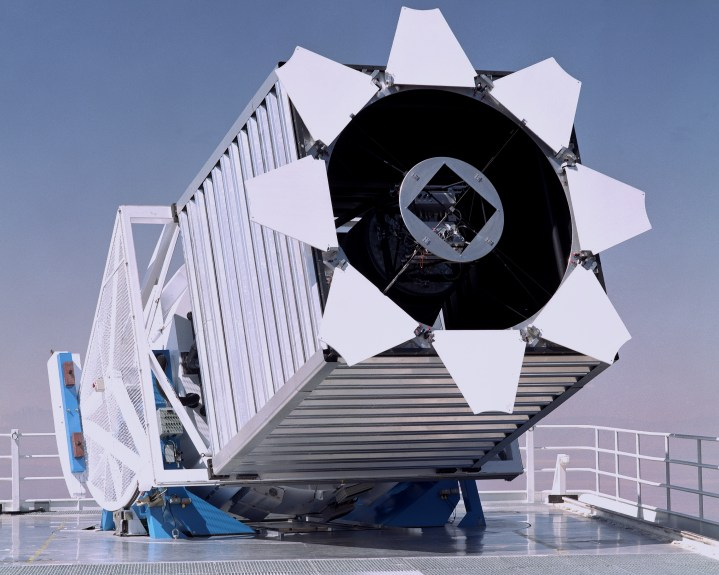
\includegraphics[height=6cm]{SDSS/sdss_telescope.jpg}~%
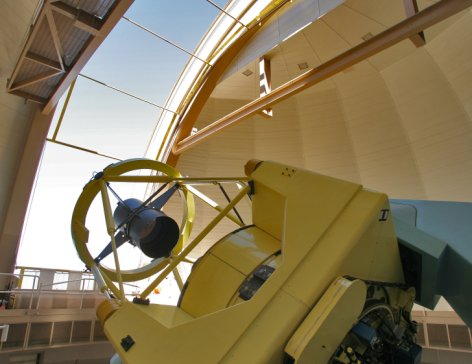
\includegraphics[height=6cm]{SDSS/IDP_Chile.jpg}
\caption{\textbf{Left:} The Apache Point Observatory's $2.5~m$ telescope. \textbf{Right:} The Las Campanas Observatory's $2.5~m$ telescope. Credit: SDSS}
\label{fig:apo_telescope}
\end{center}
\end{figure}


At the conclusion of the first and second generations in 2008 (SDSS lasting 5 years and SDSS-II lasting 3 years), the survey consisted of a $11,663~\mathrm{deg}^2$ photometric survey of in $5$ wavelength bands along with a spectroscopic survey of $1,640,960$ spectra, including over $930,000$ galaxies, $120,000$ quasars and $460,000$ stars. The astrometric data from the
photometric survey along with the redshifts measured in the spectroscopic data made it possible to map out a three-dimensional region of the Universe, all made publicly available in the seventh data release\footnote{\url{http://www.sdss.org/dr7}} (DR7). This unprecedently large data set has had a consequential
impact on our knowledge of both astrophysics and cosmology, one of the most famous results being
the first ever detection of Baryon Acoustic Oscillations (BAOs, Sec.~\ref{sec:baos}) by \cite{Eisenstein2005} using a sample of $\sim 46,000$ Luminous Red Galaxies (LRGs), allowing a measurement of absolute distance at $z=0.35$ with a precision of $5\%$. \\

Directly following SDSS-II, SDSS-III started in 2008 using the same telescope, and consisted of $4$
different surveys: \\
\begin{itemize}
\item[$\bullet$] the Apache Point Observatory Galactic Evolution Experiment\footnote{\url{http://www.sdss.org/surveys/apogee/}} (APOGEE), \\
\item[$\bullet$] the Multi-object APO Radial Velocity Exoplanet Large-area Survey\footnote{\url{http://www.sdss.org/surveys/marvels/}} (MARVELS), \\
\item[$\bullet$] the Sloan Extension for Galactic Understanding and Exploration 2 (SEGUE-2), and \\
\item[$\bullet$] the Baryon Oscillation Spectroscopic Survey\footnote{\url{http://www.sdss.org/surveys/boss/}} (BOSS).\\
\end{itemize}

BOSS mapped out the distribution of LRGs and quasars to measure the characteristic BAO scale. It operated from Autumn 2009 to Spring 2014 and has scanned $\sim 10,000~\mathrm{deg}^2$ of sky on a footprint that extends both in the northern and southern galactic caps. The instrument comprises of two identical spectrographs of resolution power $R \sim 2,000$ that have inherited some of the technologies developed for the first two generations of SDSS~\citep{Smee2013}. Once a list of targets has been established using photometry, a circular $0.8~m$ wide $3.2~mm$ thick Aluminium plate destined to lie at the focal plane of the Apache Point telescope is drilled with $\sim 1,000$ holes on which are plugged a bundle of optical fibers to the spectrograph during nights of spectroscopic observations. This enables getting the spectra of several hundreds of objects simultaneously and with the same observational conditions in wavelengths $3,600 \leqslant \lambda / {\AA} \leqslant 10,500$. The fibers are $180 ~\mu m$ in diameter each and cover a $3''$ area of sky. The entire plate covers a $5~\mathrm{deg}^2$ patch of sky. Each object is usually observed between $5$ and $9$ times and so the spectra are co-added to reduce the signal-to-noise ratio. Our working group in Saclay is involved in the BOSS as well as its successor, the Extended Baryon Oscillations Spectroscopic Survey (eBOSS) in the fourth and current generation of SDSS (SDSS-IV) operating from 2014 to 2020;  and the Dark Energy Spectroscopic Instrument (DESI). We are mainly involved in the target selection~\citep{Ross2012, Raichoor17}, quasar clustering and measurement of the 2-point correlation function~\citep{PierreLaurent1, PierreLaurent2}, the quasar luminosity function~\citep{QSO_luminosity_function}, redshift-space distortions~\citep{RSD}, and Ly-$\alpha$ forests.\\

\begin{figure}
\begin{center}
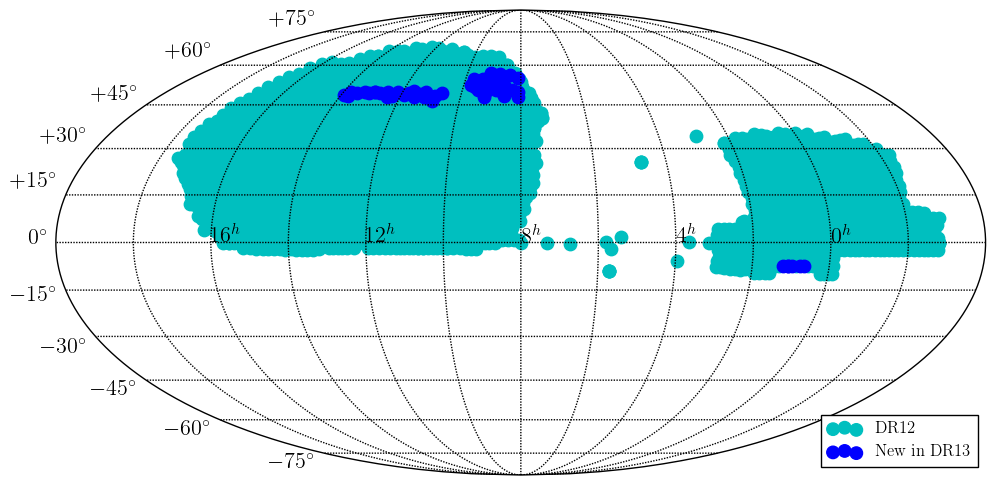
\includegraphics[height=4.5cm]{SDSS/dr13_boss.png}~%
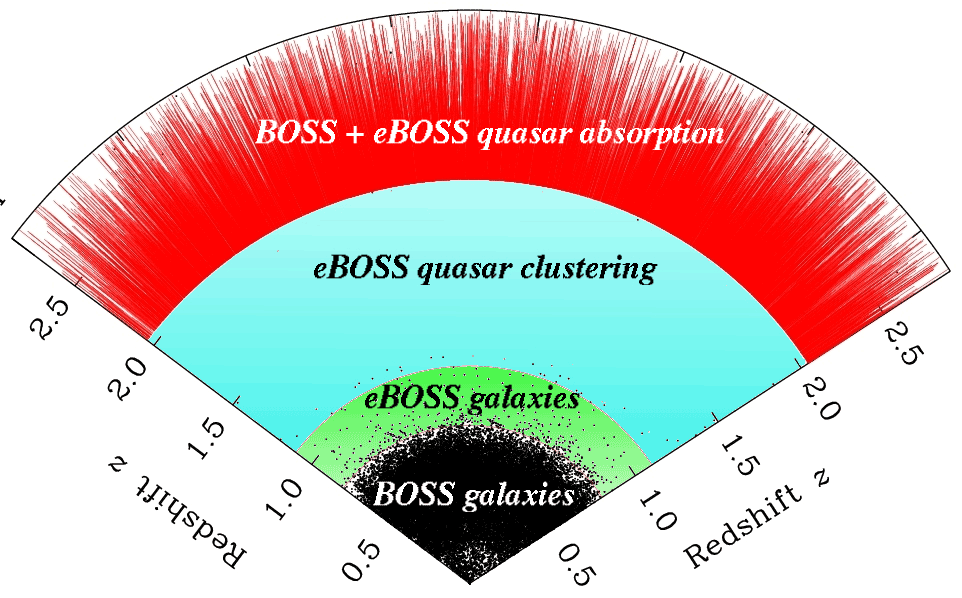
\includegraphics[height=4.5cm]{SDSS/pie_boss_eboss_marked.png}
\caption{\textbf{Left:} Mollweide porjection of the angular footprint of eBOSS in the Earth's coordinate system. \textbf{Right:} BOSS and eBOSS surveys outline of their respective depth in redshift. Credit: SDSS-IV/eBOSS}
\label{fig:bosseboss}
\end{center}
\end{figure}


Nowadays, SDSS-IV consists of the second chapter of APOGEE, the aforementionned extension of BOSS and the Mapping Nearby Galaxies at APO (MaNGA) survey\footnote{\url{http://www.sdss.org/surveys/manga/}}. eBOSS (see Fig.~\ref{fig:bosseboss}) uses the same spectrographs and aims at the measurement of the BAO scale at $0.6 \leqslant z \leqslant 2.5$, $375,000$ LRGs over $7,500~\mathrm{deg}^2$ from $z=0.6$ to $0.8$, $260,000$ Emission Line Galaxies (ELGs) over $1,500~\mathrm{deg}^2$ from $z=0.6$ to $1.0$ and $740,000$ quasars over $7,500~\mathrm{deg}^2$ from $z=0.9$ to $3.5$. As of the most current (12$^{\mathrm{th}}$, 13$^{\mathrm{th}}$) data releases, there are $297,301$ catalogued quasars~\citep{DR12Q_catalogue}. For my PhD work, I used the previous quasar catalog from the ninth data release \citep{DR9Q_catalogue} which comprises $87,822$ quasars detected over $3,275~\mathrm{deg}^2$. 




\subsubsection{SDSS/BOSS Ly-$\alpha$ power spectrum}

The 1D power spectrum had been measured by \cite{McDonald2006} using $3,035$ Ly-$\alpha$ forests from the seventh data release of SDSS~\citep{York2000, SDSSDR7}. This DR7 power spectrum was measured in $9$ redshift bins from $\langle z \rangle = 2.2$ to $3.8$ with step $\Delta z = 0.2$ and in $12$ $k$ mode bins from $k=1.41 \times 10^{-3}$ to $1.778 \times 10^{-2}~s~\rm{km}^{-1}$ of constant logarithmic step $\Delta \log (k/s~\mathrm{km}^{-1}) \simeq 0.1$. Here, the quantity is defined as $k = 2 \pi / v$ where $v$ is the wavelength of a Fourier mode and is measured in $\mathrm{km}/s$. It should not be confused with the spectral wavelength $\lambda/\lambda_0 = \exp \left[ \Delta v / c \right]$. It was at the time almost 2 orders of magnitude larger than any previously available data set, with a statistical uncertainty of $\sim 0.6~\%$ on the overall amplitude of the power spectrum. \\

In \cite{Palanque-Delabrouille2013}, we presented the measurement of the 1D power spectrum using $13,821$ Ly-$\alpha$ forests from the parent sample of $\sim 90,000$ quasar spectra of the ninth data release of SDSS-III/BOSS~\citep{Ahn2012, Dawson2012, Eisenstein2011, Gunn2006, Ross2012, Smee2013}, selected for the following criteria on their Ly-$\alpha$ forest: \\

\begin{itemize}
\item[$\bullet$] a signal-to-noise ratio per $\Delta \lambda / \lambda = 10^{-4}$ pixel greater than 2, \\
\item[$\bullet$] absence of broad absorption line (BALs) features, \\
\item[$\bullet$] absence of damped or detectable Lyman-limit systems (DLA), and \\
\item[$\bullet$] an average resolution in the Ly-$\alpha$ forest of at most $85~\rm{km}~s^{-1}$.\\
\end{itemize}

We use this Ly-$\alpha$ forest sample to compute the QSO--Ly-$\alpha$ cross-correlation as well as the Ly-$\alpha$ auto-correlation, which is my line of work. We measure the transmitted flux power spectrum in $12$ redshift bins from $\langle z \rangle = 2.2$ to $4.4$ of step $\Delta z = 0.2$ and in $35$ $k$ bin modes ranging from $k=1.084 \times 10^{-3}$ to $1.9512 \times 10^{-2}~s~\rm{km}^{-1}$ of constant step $\Delta k = 5.42 \times 10^{-4}s~\mathrm{km}^{-1}$. To reduce correlations between neighboring $z$-bins, we split the Ly-$\alpha$ forest of each quasar spectrum into up to three distinct redshift sectors. Each sector has a maximum extent of $\Delta z < 0.2$. The transmitted flux power spectrum $\vert \tilde{\delta_\varphi}(k) \vert^2$ is computed separately in each $z$-sector. We checked that the resulting power spectrum agreed with that derived from a likelihood approach. Complete details on our selection procedure as well as calibrations, computation of the flux power spectrum and  determination of both statistical and systematic uncertainties are extensively described in~\cite{Palanque-Delabrouille2013}. \\

\begin{figure}
\begin{center}
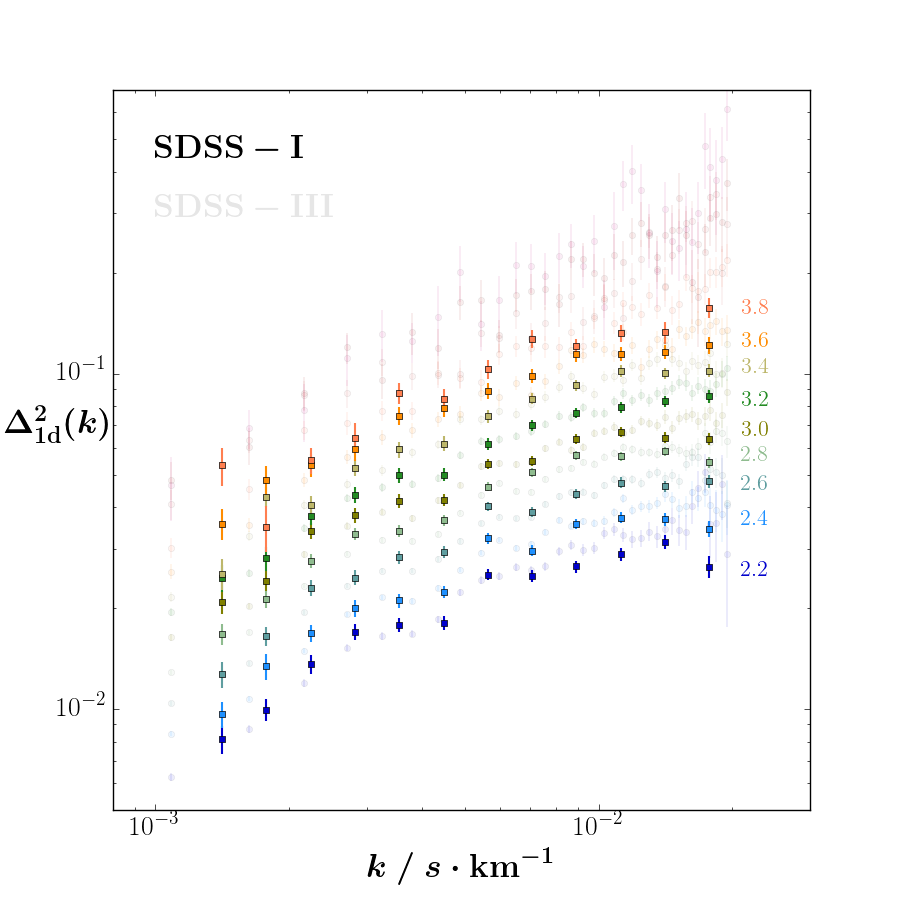
\includegraphics[width=0.7\columnwidth]{Data/Data_sdss1.png}
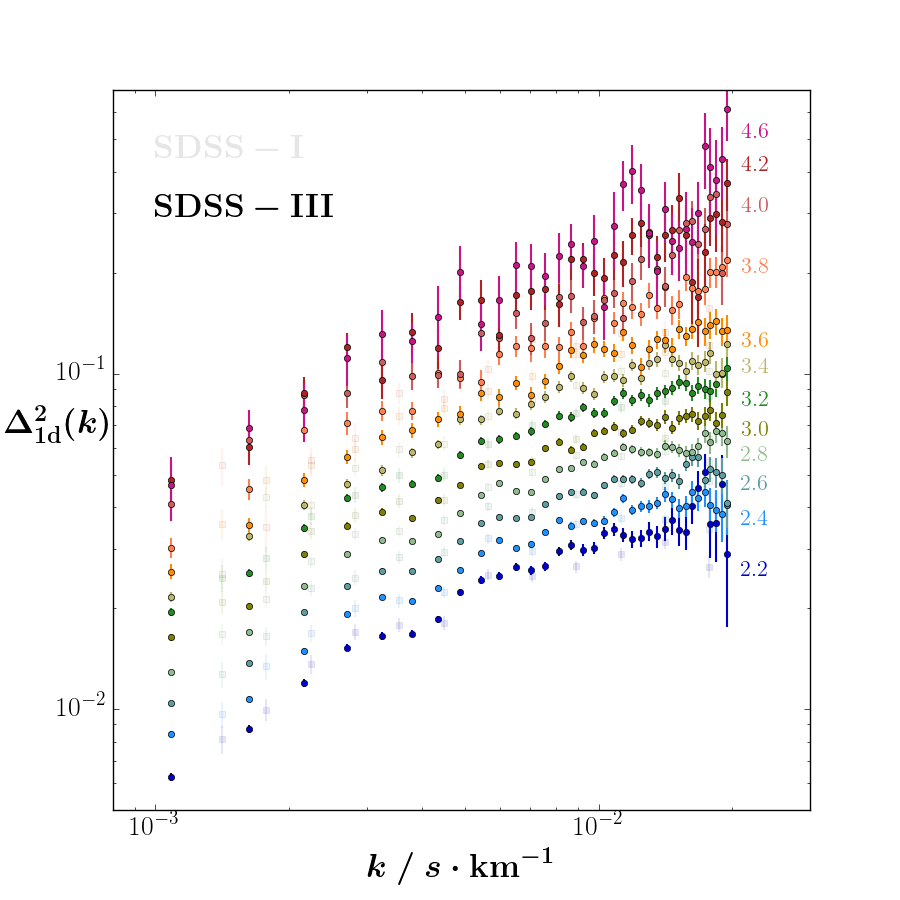
\includegraphics[width=0.7\columnwidth]{Data/Data_sdss3.png}
\caption{Adimensional Ly-$\alpha$ flux power spectrum measured with SDSS-I and SDSS-II (top) and SDSS-III (bottom). The color code corresponds to the redshift bin. Error bars are the uncertainty on the power spectrum (systematic + statistical). In each panel, the other sample is overlayed in semi-transparent to showcase the gains from the SDSS-II to the SDSS-III sample.}
\label{fig:sdss_before_after}
\end{center}
\end{figure}


Since both $1/k$ and $P_{\varphi}(k)$ are homogenous to a velocity, the quantity 
\begin{equation}
\Delta^2_{\mathrm{1d}} (k, z) \doteq \frac{k}{2 \pi} \times P_{\varphi}(k,z)
\end{equation} is dimensionless. Similarly to the dimensionless matter power spectrum in Eq.~\ref{eq:variance_ps}, it quantifies the variance per $\log_{10}k$ of the transmitted flux fraction along a line-of-sight. In Fig.~\ref{fig:sdss_before_after}, I display this adimensional flux power spectrum for both the DR7 (top panel) and our DR9 (bottom panel) samples. The addition of 3 redshift bins, a more resolute sampling of the $k$ modes and the shear number of objects in each $(k, z)$ bin make our DR9 sample far better suited to search for evidence of neutrino masses in the Ly-$\alpha$ forests of quasars. The higher the redshift bin, the more sparsely populated it is. The highest redshift bins in our survey for instance ($\langle z \rangle = 4.2, 4.4$) only contain a handful of objects, whereas the lowest ones count several thousands. This explains the larger error bars at all scales for the highest (redest) redshifts, which are dominated by the statistical uncertainty. The highest $k$ bins at any redshift are dominated by systematic uncertainties pertaining to the spectrograph resolution. The flux power spectrum quantifies the absorption of light by the neutral Hydrogen in the IGM. The cosmological scale factor increases with time, and so decreases with redshift, meaning the physical distance between objects (including neutral Hydrogen distribution overdensities) are smaller the higher the redshift, hence more Ly-$\alpha$ absorption. Moreover, at lower redshifts, a larger fraction of the IGM Hydrogen is ionized, and thus there is less neutral Hydrogen absorbing the Ly-$\alpha$ wavelengths. The combination of these two factors strengthens the overall amplitude of the power spectrum with redshift, which is visible in both Fig.~\ref{fig:sdss_before_after} and Fig.~\ref{fig:hr_mr}.


%%%%%%%%%%%%%%%%%%%%%%%%%%%%%%%%%%%%%%%%%
\subsection{Medium Resolution Sample}
%%%%%%%%%%%%%%%%%%%%%%%%%%%%%%%%%%%%%%%%%
\label{sec:mrs}

\subsubsection{The XQ-100 survey}

The Very Large Telescope (VLT) is an array of facilities of the European Southern Observatory\footnote{\url{http://www.eso.org/public/}} located on the Cerro Paranal site in Chile, altitude $2,635~m$. It consists of 4 identical Ritchey-Chr\'etien $8.2~m$ Unit Telescopes, named Antu (UT1), Kueyen (UT2), Melipal (UT3) and Yepun (UT4), the first of which began observations in Spring 1998. There are also 4 mobile $1.8~m$ Auxiliary Telescopes which, when operating in conjunction with the UTs, can form an interferometer (the ESO VLTI) which can resolve a milli-arcsecond. \\

Mounted on the Cassegrain focus of UT2 lies XSHOOTER~\citep{XShooter} ( pictured in the right panel of Fig.~\ref{fig:vlt_telescope}), an intermediate-resolution spectrograph that can cover, in a single exposure, wavelengths of $3,000 \leqslant \lambda / {\AA} \leqslant 24,800$. It consists of $4$ arms, one for aquisition and guidance, while the other $3$ are fixed echelle spectrographs\footnote{prism cross-dispersers} covering different wavelength ranges:\\

\begin{itemize}
\item[$\bullet$] UVB, covering the ultraviolet and blue $3,000 \leqslant \lambda / {\AA} \leqslant 5,595$; \\
\item[$\bullet$] VIS, covering the visible range $5,595 \leqslant \lambda / {\AA} \leqslant 10,240$; and \\
\item[$\bullet$] NIR, covering the near infrared $10,240 \leqslant \lambda / {\AA} \leqslant 24,800$. \\
\end{itemize}

\begin{figure}
\begin{center}
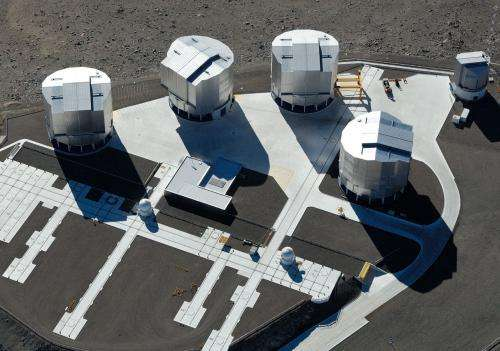
\includegraphics[height=5.6cm]{SDSS/VLT_UT.jpg}~%
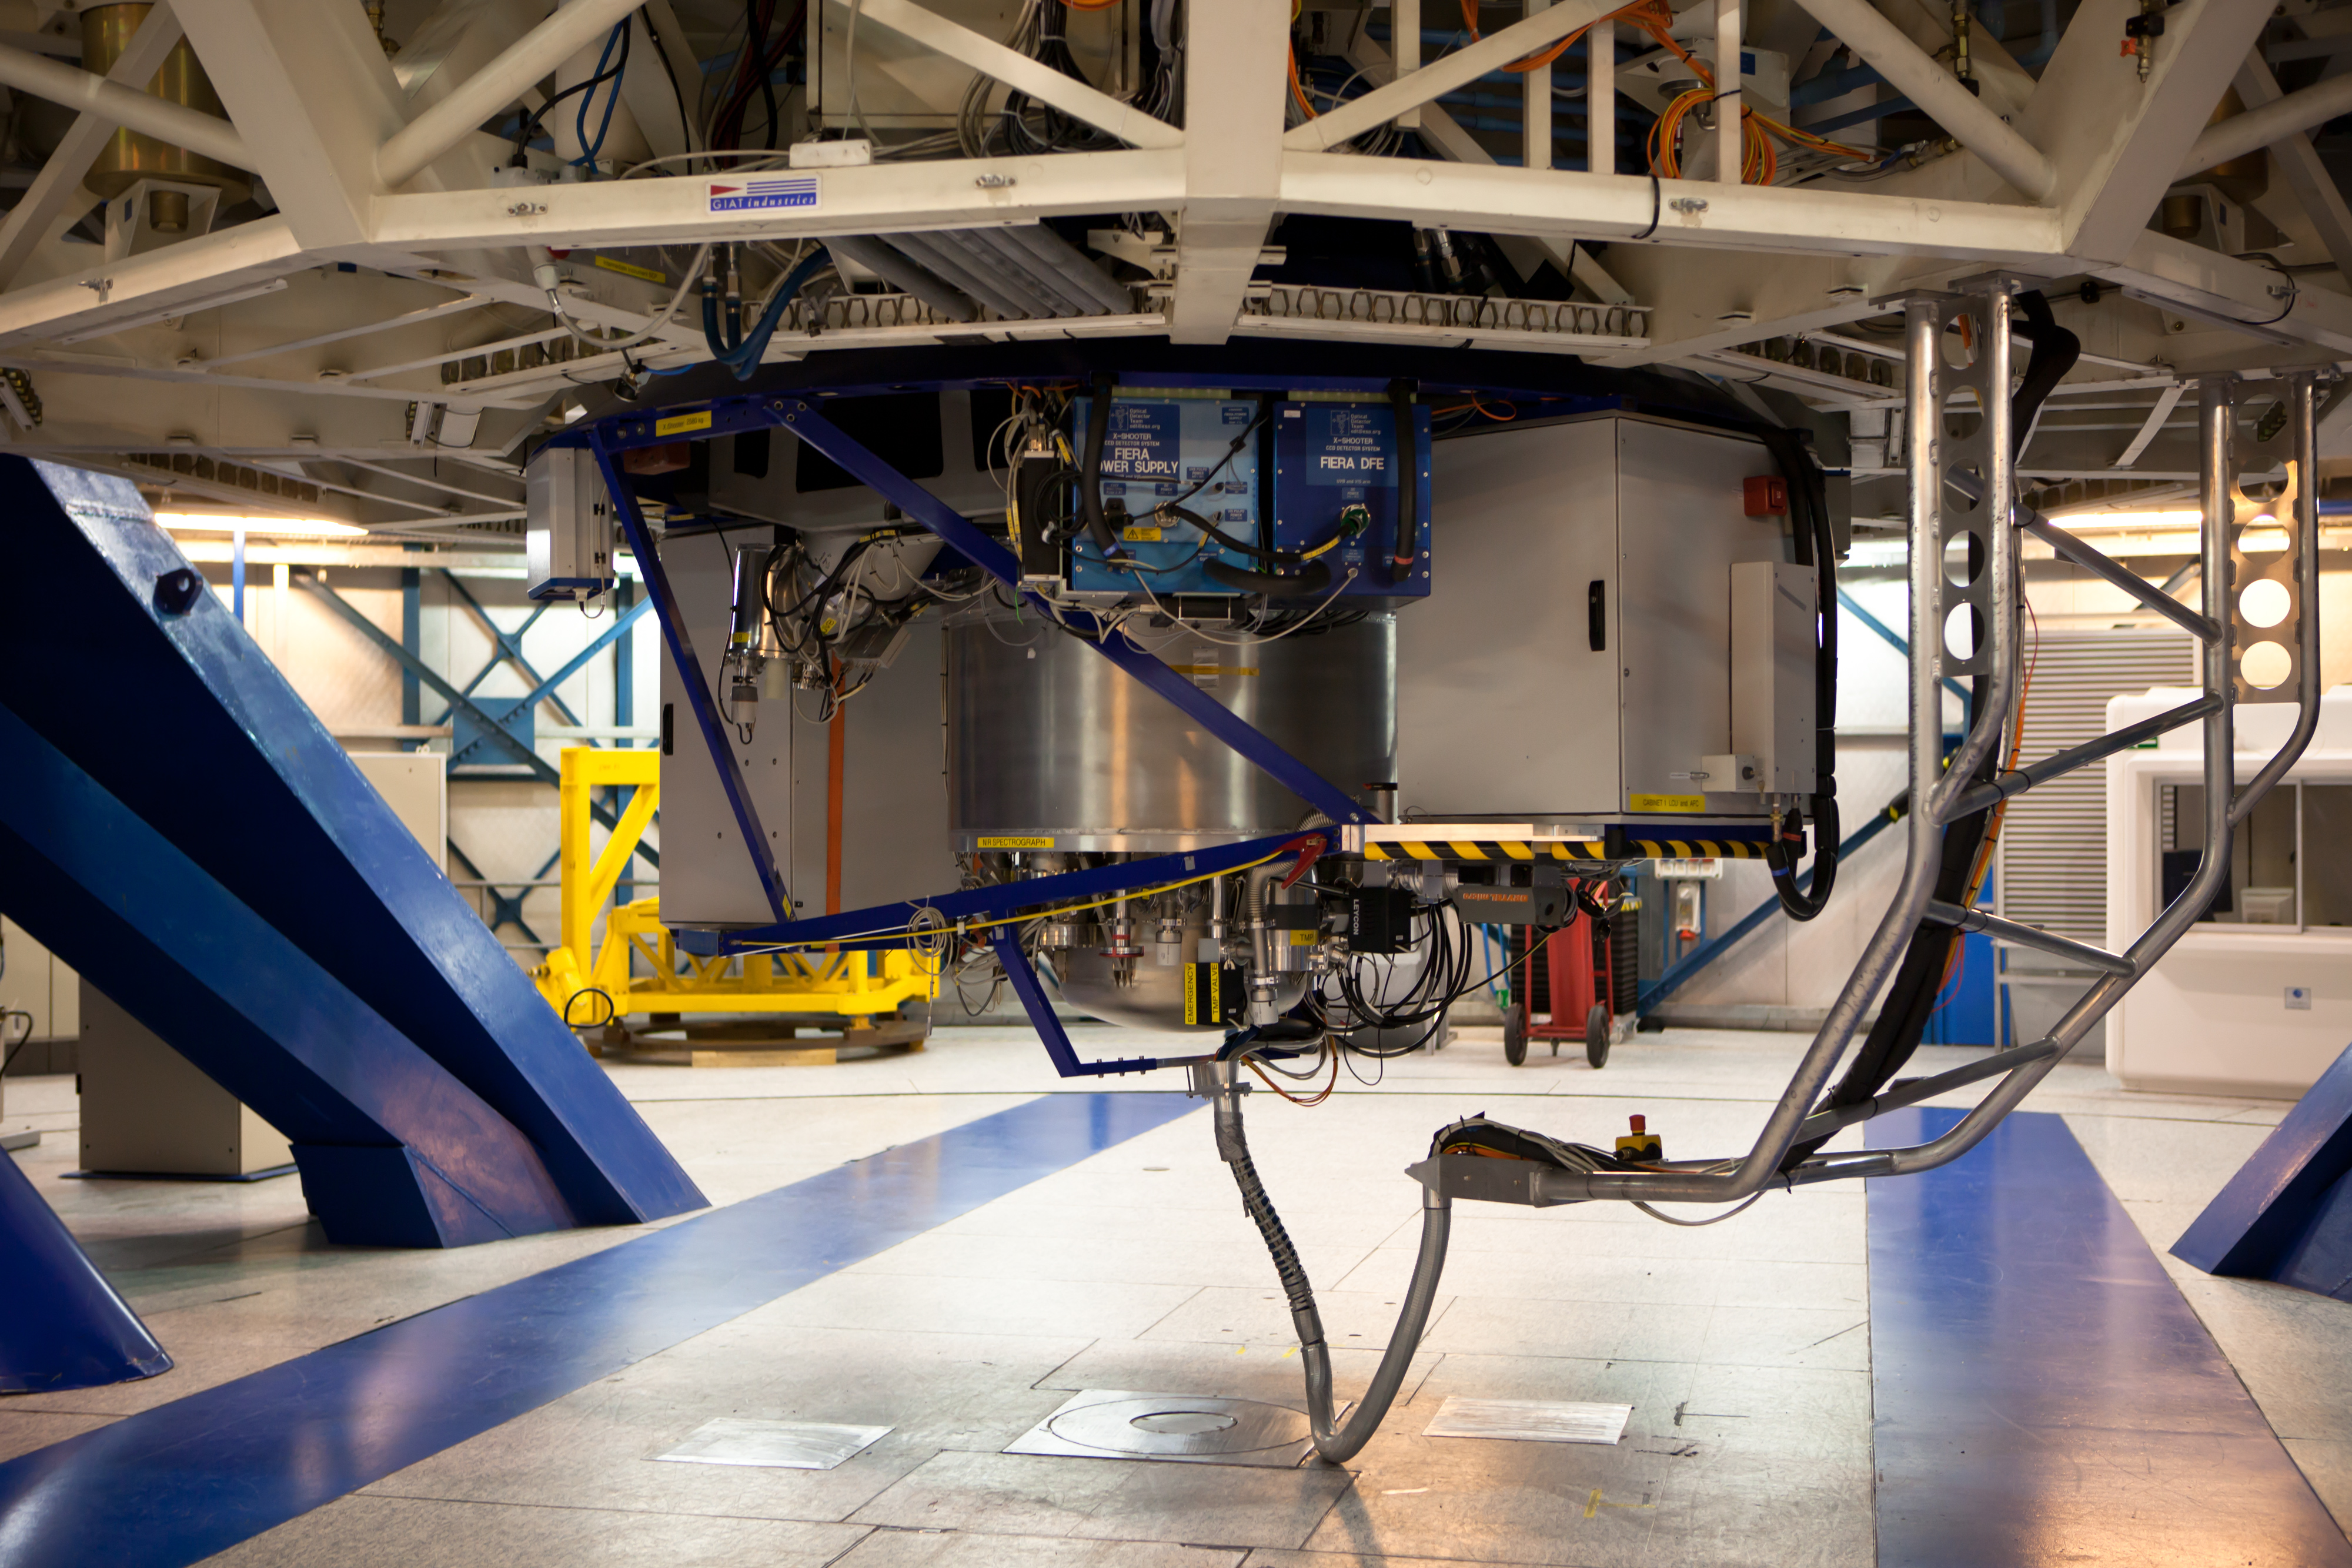
\includegraphics[height=5.6cm]{SDSS/XShooter.jpg}
\caption{\textbf{Left:} The Very Large Telescope's four $8.2~m$ Unit Telescopes. \textbf{Right:} The XSHOOTER spectrograph mounted on UT2. Credit: ESO}
\label{fig:vlt_telescope}
\end{center}
\end{figure}


The instrument is designed to maximize the sensitivity in this spectral range through dichroic splitting in the $3$ spectroscopic arms, and operates at spectral resolutions considered intermediate: $R=4-17 \times 10^3$, depending on the spectroscopic arm (wavelength range) and the width of the slit. This is far more resolute than the BOSS spectrographs. However, only a single target can be observed during an exposure, contrary to BOSS and eBOSS which can simultaneously split the light from several hundreds of targets in the same patch of sky. A dedicated data reduction pipeline delivers fully calibrated two-dimensional and extracted spectra over the full wavelength range. \\

The XQ-100 project~\citep{XQ100} is one of the large programs of the European Southern Observatory, ``Quasars and their absorption lines: a legacy survey of the high-redshift universe with XSHOOTER released''. It consists of a homogeneous and high-quality sample of 100 echelle spectra of quasars at redshifts $z \simeq 3.5-4.5$,  observed with full spectral coverage of XSHOOTER. 


\subsubsection{XQ-100 Ly-$\alpha$ power spectrum}

\begin{figure}[!]
\begin{center}
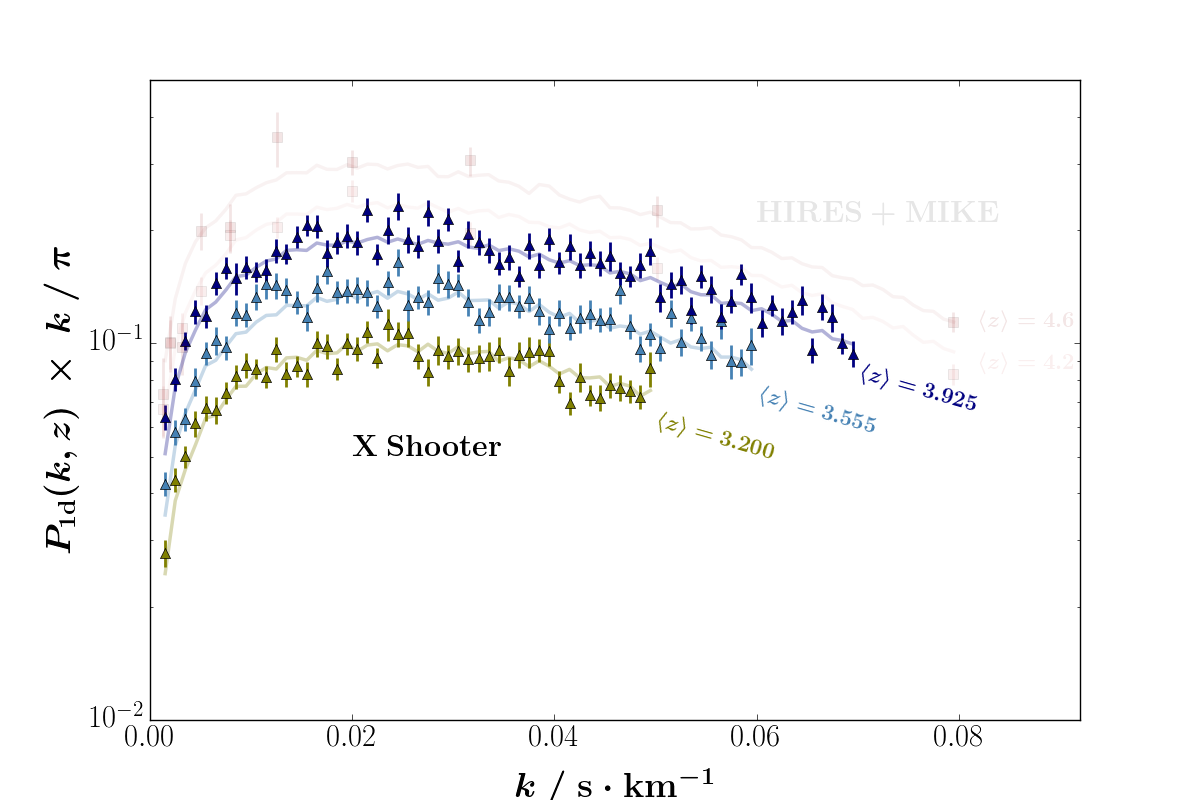
\includegraphics[width=0.85\columnwidth]{Data/XShooter.png}
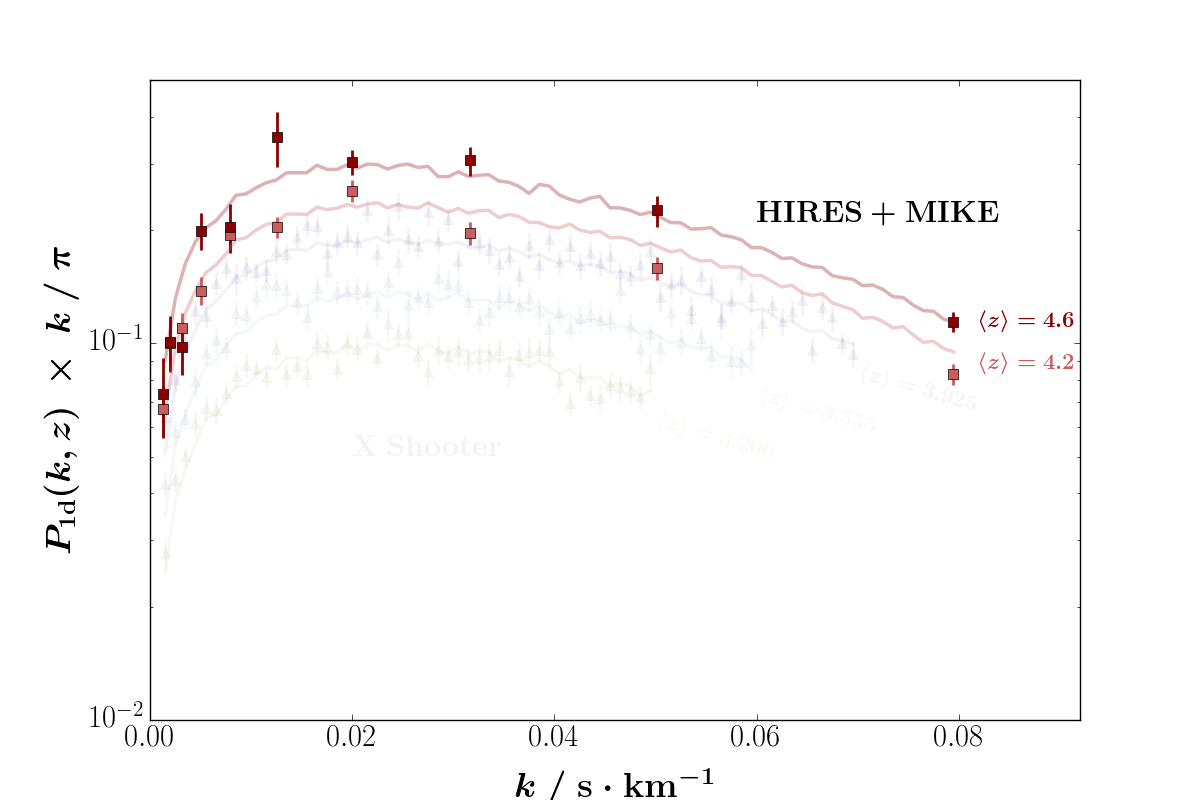
\includegraphics[width=0.85\columnwidth]{Data/HIRESMIKE.png}
\caption{Adimensional Ly-$\alpha$ flux power spectra measured with the XSHOOTER spectrograph (top) and the combined set of quasar spectra obtained from the MIKE and HIRES spectrographs (bottom). Error bars are the uncertainty on the power spectrum, as reported in their references. The solid lines correspond to the best fit models from our analysis described in Sec.~\ref{sec:methodology}.}
\label{fig:hr_mr}
\end{center}
\end{figure}

For our work on the Ly-$\alpha$ power spectrum, we make use of the XQ-100 Science Data Products (SDP) available at \url{http://archive.eso.org/wdb/wdb/adp/phase3_main/form}, specifically the VIS and UVB arms, of resolution $12~\mathrm{km}~s^{-1}$ and  $18~\mathrm{km}~s^{-1}$ respectively.  The signal-to-noise ratio per pixel in the Ly-$\alpha$ forest varies from 5 to 60, with an average of $\sim 25$. For comparative purposes, the $\sim 700$ BOSS quasars in the same \textsc{Hi} absorption region ($z \simeq 3.0-4.2$) analysed in~\cite{Palanque-Delabrouille2013} exhibit a $10-20$ times lower signal-to-noise ratio for a $3$ to $5$ times weaker spectral resolution compared to the $100$ quasar spectra in the XQ-100 survey.  Consequently, XQ-100 data allow us to reach down to scales of $7 \times 10^{-2}~s~\mathrm{km}^{-1}$ with the VIS arm which has the better resolution.\\

We measure the Ly-$\alpha$ power spectra in 70 $k$ bins for 3 redshifts centered on $\langle z \rangle = 3.200, 3.555, 3.925$ following the methodology described in \cite{Yeche17} and shown in the upper panel of Fig.~\ref{fig:hr_mr}. I overlay the dimensionless power spectra constructed with our best fit models at the 3 nearest redshift bins at which I ran hydrodynamical simulations ($z=3.2, 3.6, 4.0$). The raw power spectrum measured in these bins asymptotically approaches the noise power spectrum computed as a white noise at small scales. With a pixel size of $\Delta v = c~ \Delta \lambda / \lambda$ of $20~ \mathrm{km}~s^{-1}$ for the UVB and $11~ \mathrm{km}~s^{-1}$ for the VIS arm, the largest modes, determined by the Nyquist-Shannon limit $k_{\mathrm{Nyq}} = \pi / \Delta v$, are respectively $k_{\mathrm{Nyq}}^{\mathrm{uvb}} = 0.16~s~\mathrm{km}^{-1}$ and $k_{\mathrm{Nyq}}^{\mathrm{vis}} = 0.29~s~\mathrm{km}^{-1}$. Because of an uncertainty on the correction of the spectrograph resolution, however, we limit our study to 50, 60 and 70 $k$ bins respectively (corresponding to $k \leq 0.05, 0.06, 0.07~s~\mathrm{km}^{-1}$) for the 3 aforementionned redshifts. This screening ensures the raw power spectrum is always dominant over the noise power spectrum at these small scales. 


%%%%%%%%%%%%%%%%%%%%%%%%%%%%%%%%%%%%%%%%%%%%%%%%%
\subsection{High Resolution Samples}
%%%%%%%%%%%%%%%%%%%%%%%%%%%%%%%%%%%%%%%%%%%%%%%%%


\begin{figure}[!]
\begin{center}
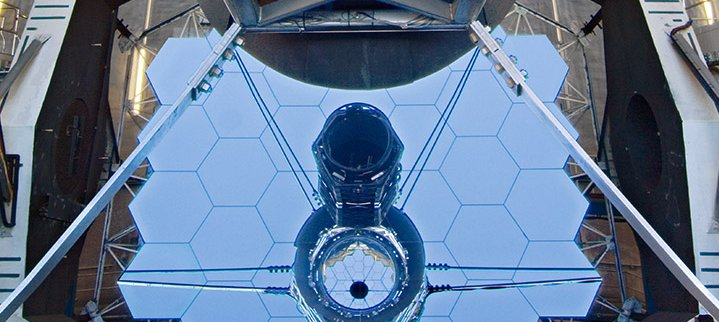
\includegraphics[height=4.5cm]{SDSS/keck.jpg}~%
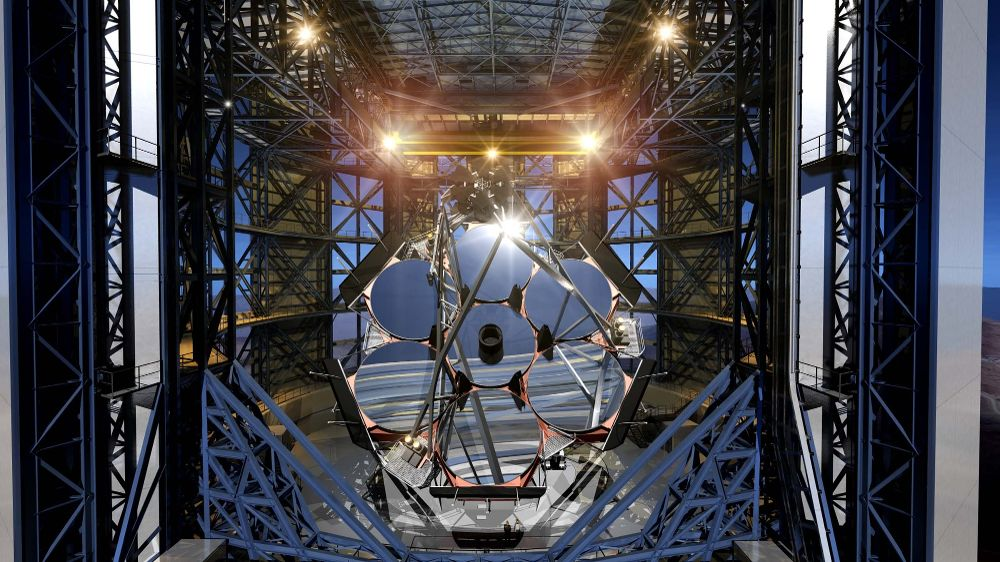
\includegraphics[height=4.5cm]{SDSS/lco_mag.jpg}
\caption{\textbf{Left:} Close-up view of the $10.0~m$ primary mirror of the W.M. Keck telescopes. Credit: WMKO, California Institute of Technology (Caltech). \textbf{Right:} Close-up view of the $6.5~m$ primary mirror of the Giant Magellan Teslescopes. Credit: LCO/GMTO.}
\label{fig:wmko_telescope}
\end{center}
\end{figure}

\subsubsection{The WMKO/HIRES spectrograph}

The William Myron Keck Observatory\footnote{url{http://www.keckobservatory.org/}} (WMKO) is one amongst the several observatories atop Hawaii's Mauna Kea volcano, elevation $4,145~m$, and is home to two identical altitude-azimuth Ritchey-Chr\'etien telescopes. They are currently amongst the largest optical telescopes in use today, and the particularity of their $10.0~m$ primary mirrors are a mosaic of $36$ hexagonal segments. They have a focal distance of $17.5~m$, giving them a $f/1.75$ focal to aperture ratio. They began operations in 1990 and 1996. Mounted permanently on the right Nasmyth platform of one of the Keck telescopes rests the High Resolution Echelle Spectrometer, HIRES~\citep{HIRES}. It is a grating cross-dispersed, echelle spectrograph that spans the $3,000 \leqslant \lambda / {\AA} \leqslant 10,000$ wavelength range and attains resolutions of $R=25-85 \times 10^3$ depending on the slit of choice.



\subsubsection{The LCO/MIKE spectrograph}

In addition to the aforementioned Ir\'en\'ee du Pont telescope, the Las Campanas Observatory also houses two $6.5~m$ Magellan telescopes, Baade and Clay, which saw first light is 2000 and 2002. Each Magellan telescope's main mirror is a $f/1.25$ paraboloid made of 7 circular mirrors, pictured in the right panel of Fig.~\ref{fig:wmko_telescope}. In 2002, the Magellan Inamori Kyocera Echelle (MIKE) spectrometer~\citep{MIKE} was installed on Clay. It is a double echelle spectrograph that spans the $3,350 \leqslant \lambda / {\AA} \leqslant 5,000$ blue and $4,900 \leqslant \lambda / {\AA} \leqslant 9,500$ red ranges.

\subsubsection{MIKE+HIRES Ly-$\alpha$ power spectrum}

The high-resolution LCO/MIKE and WMKO/HIRES spectrographs yield the highest resolution quasar spectra available. \cite{HRdata} measured the power spectrum is measured in 4 redshift bins ($\langle z \rangle = 4.2, 4.6, 5.0, 5.4$) and 9 $k$ bins spanning down to $k \leq 0.08~ s~\mathrm{km}^{-1}$. In our work on the Ly-$\alpha$ power spectrum, we compute the theoretical  power spectrum from $z=4.6$ downwards. Therefore, we can only make use of the two lower $z$ bins for this data set, which I plot on the bottom panel of Fig.~\ref{fig:hr_mr} along with our best fitted power spectrum at the corresponding redshifts. 
